\documentclass[aspectratio=169]{beamer}
\usepackage{graphicx}
\usepackage{hyperref}
\usetheme{metropolis}
\title{Decision and RAID Logs}
\institute{Engineers for Exploration, UC San Diego}
\logo{
\includegraphics[height=.65cm,keepaspectratio]{e4e_logo_350x136.png}}
\setbeamertemplate{caption}[numbered]
\begin{document}
\maketitle
\begin{frame}{Obligatory Comic}
    \centering
    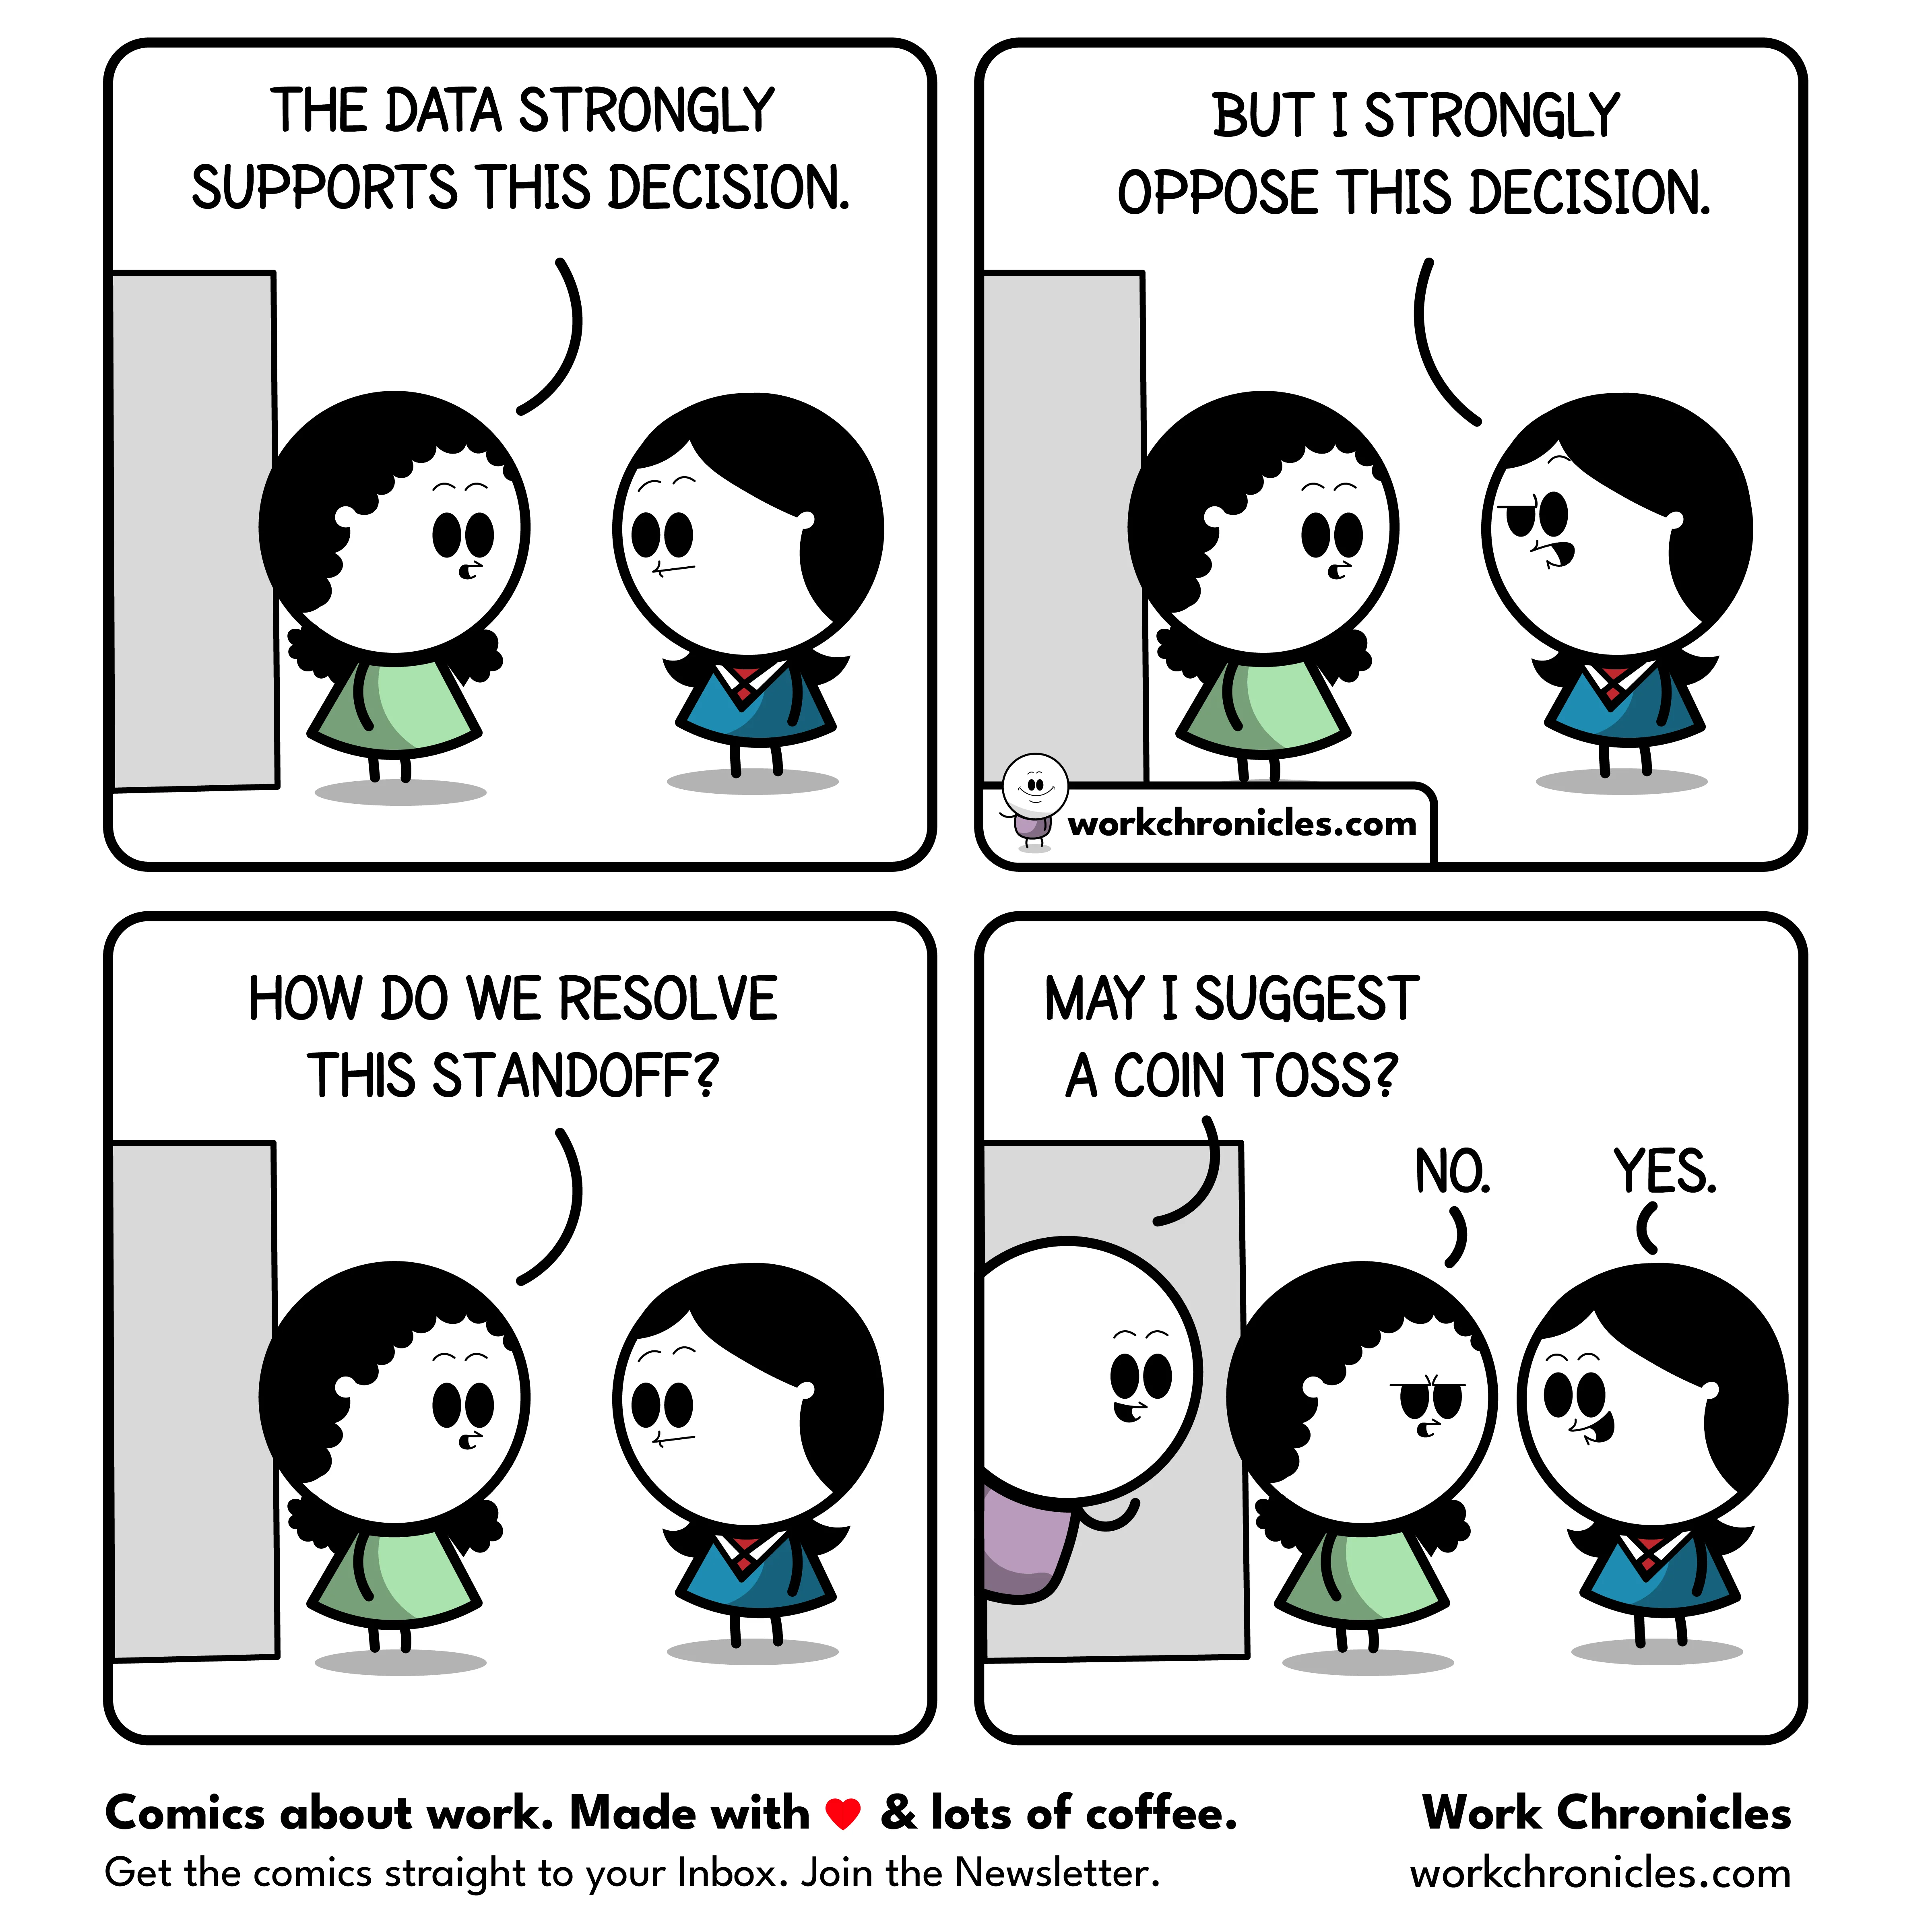
\includegraphics[width=0.8\textwidth,height=0.8\textheight,keepaspectratio]{15_decision_comic.png}
\end{frame}
\begin{frame}{Why do we need to keep track of decisions?}
    \begin{itemize}[<+->]
        \item Get buy in from everyone
        \item Remember why we did something in the future
        \item Communicate decisions to the rest of the team
    \end{itemize}
\end{frame}
\begin{frame}{What kinds of decisions do we log?}
    \begin{itemize}[<+->]
        \item Critical decisions
        \item Course of action decisions
        \item Risk management decisions
        \item Project team decisions
        \item Deliverables decisions
        \item Metrics and evaluation decisions
    \end{itemize}
\end{frame}
\begin{frame}{What do we log?}
    \begin{itemize}
        \item Decision details
        \item Decision maker
        \item Stakeholders involved
        \item Rationale
        \item Follow-up actions
    \end{itemize}
\end{frame}
\begin{frame}{What is a RAID log?}
    \begin{itemize}
        \item Risks
        \item Assumptions
        \item Issues
        \item Dependencies
        \item Actions
        \item Decisions
    \end{itemize}
\end{frame}
\begin{frame}{RAID Log Example 1}
    \centering
    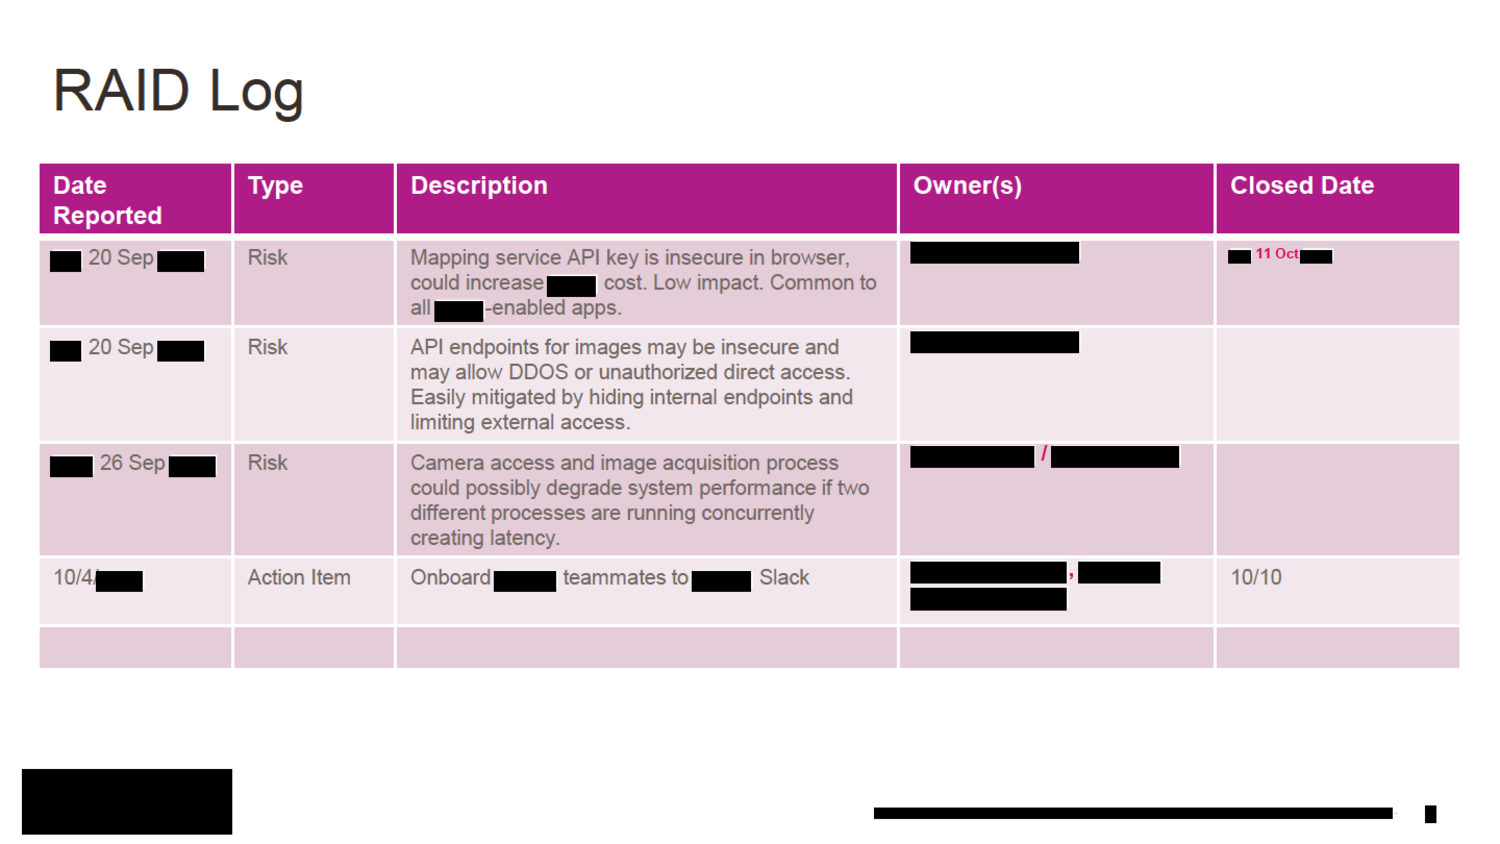
\includegraphics[width=0.8\textwidth,height=0.8\textheight,keepaspectratio]{15_raid_log_example.pdf}
\end{frame}
\begin{frame}{RAID Log Example 2}
    \begin{enumerate}
        \item Risks
        \begin{enumerate}
            \item Fabric store doesn't have enough material:
            \begin{enumerate}
                \item Solution A: Inquire whether the store can order more of the preferred material within the deadline.
                \item Solution B: Try another local fabric store for the same or similar material.
                \item Solution C: Choose a complementary fabric and use both for upholstery.
                \item Solution D: Use a different fabric for the project.
            \end{enumerate}
            \item Need different tools from those expected:
            \begin{enumerate}
                \item Solution A: Ask if a colleague has the proper tools.
                \item Solution B: Visit a hardware store to purchase tools.
                \item Solution C: Order tools online
            \end{enumerate}
        \end{enumerate}
    \end{enumerate}
\end{frame}
\begin{frame}{RAID Log Example 2 (continued)}
    \begin{enumerate}
        \setcounter{enumi}{1}
        \item Assumptions
        \begin{enumerate}
            \item Upholstery project only applies to the five chairs in the current dining room set
            \begin{itemize}
                \item Validity assessment: Ask the client to confirm upholstery project doesn't extend to extra chairs kept in storage.
                \item Plan if the client extends the project: Ask the client about the number of chairs for the project and plan to order additional materials to compensate for the extra chairs.
            \end{itemize}
        \end{enumerate}
        \item Issues
        \begin{enumerate}
            \item Discovered instability in legs of one chair
            \begin{itemize}
                \item Resolved issue Monday afternoon by replacing screws.
            \end{itemize}
        \end{enumerate}
        \item Dependencies
        \begin{enumerate}
            \item Fabric store stock
            \item Client deadline
            \item Initial structural integrity of chairs
            (Dependency added to account for extra work completed to repair damaged chair legs.)
        \end{enumerate}
    \end{enumerate}
\end{frame}
\end{document}